\documentclass[aspectratio=169, 12pt]{beamer}

% ── Theme ─────────────────────────────────────────────────────────────────────
\usetheme{Madrid}
\usecolortheme{seahorse}
\setbeamertemplate{navigation symbols}{}
\setbeamertemplate{footline}[frame number]

% ── Packages ──────────────────────────────────────────────────────────────────
\usepackage{amsmath, amssymb}
\usepackage{graphicx}
\usepackage{booktabs}
\usepackage{xcolor}
\usepackage{tikz}
\usepackage{listings}

\graphicspath{{../../plots/}}

% ── Custom colors ─────────────────────────────────────────────────────────────
\definecolor{trivial}{HTML}{d62728}
\definecolor{critical}{HTML}{2ca02c}
\definecolor{topological}{HTML}{1f77b4}
\definecolor{edgemode}{HTML}{e377c2}
\definecolor{codebg}{HTML}{f5f5f5}
\definecolor{codekw}{HTML}{0000cd}
\definecolor{codecomment}{HTML}{228b22}
\definecolor{codestring}{HTML}{8b0000}

% ── Code listing style ────────────────────────────────────────────────────────
\lstset{
  language=Python,
  basicstyle=\ttfamily\footnotesize,
  keywordstyle=\color{codekw}\bfseries,
  commentstyle=\color{codecomment}\itshape,
  stringstyle=\color{codestring},
  backgroundcolor=\color{codebg},
  frame=single,
  framerule=0.4pt,
  rulecolor=\color{gray},
  showstringspaces=false,
  breaklines=true,
  tabsize=4,
}

% ── Macros ────────────────────────────────────────────────────────────────────
\newcommand{\cdag}{c^{\dagger}}
\newcommand{\winding}{\nu}
\newcommand{\ket}[1]{|#1\rangle}
\newcommand{\bra}[1]{\langle#1|}

% ── Title ─────────────────────────────────────────────────────────────────────
\title[Kitaev Chain — Block 2]{Majorana Modes in the Machine}
\subtitle{Block 2: The Qubit Encoding}
\author{Dobromir Stoev\\ Edgar Harutyunyan\\ Guilherme Schewtschik\\ Jaskaran Singh\\ Zhengyi Liu\\ Zhenming Shi}
\institute{Advanced Seminar — AI-Augmented Theoretical Physics}
\date{\today}

% ══════════════════════════════════════════════════════════════════════════════
\begin{document}

\begin{frame}
  \titlepage
\end{frame}

\begin{frame}{Outline}
  \tableofcontents
\end{frame}

% ══════════════════════════════════════════════════════════════════════════════
\section{Jordan-Wigner Transform}

\begin{frame}{Why map fermions to qubits?}
  \begin{columns}[T]
    \begin{column}{0.55\textwidth}
      \textbf{Goal:} simulate the Kitaev chain on a quantum computer.\\[6pt]
      Quantum computers operate on \textbf{qubits} (two-level systems),
      not directly on fermions.\\[6pt]
      \textbf{Problem:} fermionic operators anticommute,
      qubit operators on different sites commute.
      \begin{equation*}
        \{c_i, c_j^\dagger\} = \delta_{ij} \quad \text{vs} \quad
        [\sigma_i^\alpha, \sigma_j^\beta] = 0 \; (i \neq j)
      \end{equation*}
    \end{column}
    \begin{column}{0.42\textwidth}
      \begin{block}{Jordan-Wigner solution}
        Attach a \textbf{string} of $Z$ operators to each fermionic
        operator. The string encodes the fermion occupancy of all
        preceding sites and restores the correct anticommutation.
      \end{block}
    \end{column}
  \end{columns}
\end{frame}

\begin{frame}{The Jordan-Wigner mapping}
  \begin{equation}
    c_j = \underbrace{\Bigl(\prod_{k=0}^{j-1} Z_k\Bigr)}_{\text{JW string}}
          \sigma_j^-, \qquad
    c_j^\dagger = \Bigl(\prod_{k=0}^{j-1} Z_k\Bigr) \sigma_j^+
  \end{equation}
  where $\sigma^{\pm} = \tfrac{1}{2}(X \pm iY)$ are the qubit raising/lowering
  operators and $Z_k$ acts only on qubit $k$.

  \vspace{-0.5em}
  \begin{columns}[T]
    \begin{column}{0.48\textwidth}
      \textbf{Key identities}
      \begin{align*}
        c_j^\dagger c_j &= \frac{I - Z_j}{2} \quad \text{(number op.)}\\
        c_j^\dagger c_{j+1} + \mathrm{h.c.}
          &= -\frac{X_j X_{j+1} + Y_j Y_{j+1}}{2}\\
        c_j^\dagger c_{j+1}^\dagger + \mathrm{h.c.}
          &= -\frac{X_j X_{j+1} - Y_j Y_{j+1}}{2}
      \end{align*}
    \end{column}
    \begin{column}{0.48\textwidth}
      \begin{alertblock}{Why the string works}
        \small
        $Z_k$ flips sign when site $k$ is occupied.
        For $i < j$: $(c_i^\dagger)(c_j)$ picks up
        $Z_i \cdots Z_{j-1}$ from the JW string of $c_j$,
        turning commutation into \emph{anti}commutation.
      \end{alertblock}
    \end{column}
  \end{columns}
\end{frame}

% ══════════════════════════════════════════════════════════════════════════════
\section{Kitaev Hamiltonian in Qubit Language}

\begin{frame}{Substituting JW into $H_K$}
  Applying the identities to each term of
  $H_K = -\mu\sum_j\cdag_j c_j
         -t\sum_j(\cdag_j c_{j+1}+\mathrm{h.c.})
         +\Delta\sum_j(\cdag_j\cdag_{j+1}+\mathrm{h.c.})$:

  \vspace{-0.5em}
  \begin{equation}
    \boxed{
    H_K = -\frac{\mu}{2}\sum_j Z_j
          + \frac{t-\Delta}{2}\sum_j X_j X_{j+1}
          + \frac{t+\Delta}{2}\sum_j Y_j Y_{j+1}
    }
  \end{equation}

  \vspace{-0.5em}
  \begin{columns}[T]
    \begin{column}{0.48\textwidth}
      \textbf{Structure}
      \begin{itemize}
        \item $\mu$ $\to$ \textbf{transverse field} ($Z$ terms)
        \item Hopping $t$ $\to$ $XX+YY$ (number-conserving)
        \item Pairing $\Delta$ $\to$ $XX-YY$ (number-breaking)
      \end{itemize}
    \end{column}
    \begin{column}{0.48\textwidth}
      \begin{block}{Sweet spot $t = \Delta$}
        The $XX$ terms cancel.
        \[
          H = -\frac{\mu}{2}\sum_j Z_j + t\sum_j Y_j Y_{j+1}
        \]
        A pure transverse-field + $YY$ model.
      \end{block}
    \end{column}
  \end{columns}
\end{frame}

% ══════════════════════════════════════════════════════════════════════════════
\section{Fermion Parity \& Topological Degeneracy}

\begin{frame}{Fermion parity is conserved}
  The \textbf{fermion parity operator}
  \begin{equation}
    P = \prod_{j=0}^{L-1} Z_j, \qquad P^2 = I, \quad [H_K, P] = 0
  \end{equation}
  splits the $2^L$-dimensional Hilbert space into two sectors:
  \begin{itemize}
    \item \textbf{Even} parity ($P = +1$): even number of fermions
    \item \textbf{Odd} parity ($P = -1$): odd number of fermions
  \end{itemize}

  \medskip
  \begin{block}{Topological degeneracy in the qubit language}
    In the topological phase the Majorana zero modes hybridize the two parity
    sectors. The lowest even- and odd-parity states become
    \textbf{degenerate} — the \emph{parity gap} $|E_0^{(+)} - E_0^{(-)}| \to 0$.\\[4pt]
    This gap is exactly the Majorana hybridization splitting $E_0(L)$
    from Block 1, now visible as a \emph{spectral} signature in qubit space.
  \end{block}
\end{frame}

% ══════════════════════════════════════════════════════════════════════════════
\section{Numerical Verification}

\begin{frame}[fragile]{Building the qubit Hamiltonian in code}
  \begin{lstlisting}[basicstyle=\ttfamily\scriptsize]
def kitaev_qubit_hamiltonian(L, t=1.0, mu=0.0, delta=1.0):
    dim = 2 ** L
    H = np.zeros((dim, dim), dtype=complex)

    for j in range(L):
        H -= (mu / 2) * pauli_at(Z, j, L)         # transverse field

    for j in range(L - 1):
        H += ((t - delta) / 2) * two_site(X, X, j, L)   # XX coupling
        H += ((t + delta) / 2) * two_site(Y, Y, j, L)   # YY coupling

    return H
  \end{lstlisting}

  \vspace{-0.5em}
  \begin{block}{Tensor-product helpers}
    \small
    \texttt{pauli\_at(op, j, L)} embeds a single-site Pauli at site $j$ via
    $I \otimes \cdots \otimes \mathrm{op}_j \otimes \cdots \otimes I$.
    \texttt{two\_site(A, B, j, L)} places $A_j \otimes B_{j+1}$.
    Both are thin wrappers around \texttt{np.kron}.
  \end{block}
\end{frame}

\begin{frame}{Parity gap (qubit) vs BdG splitting — cross-check}
  \begin{center}
    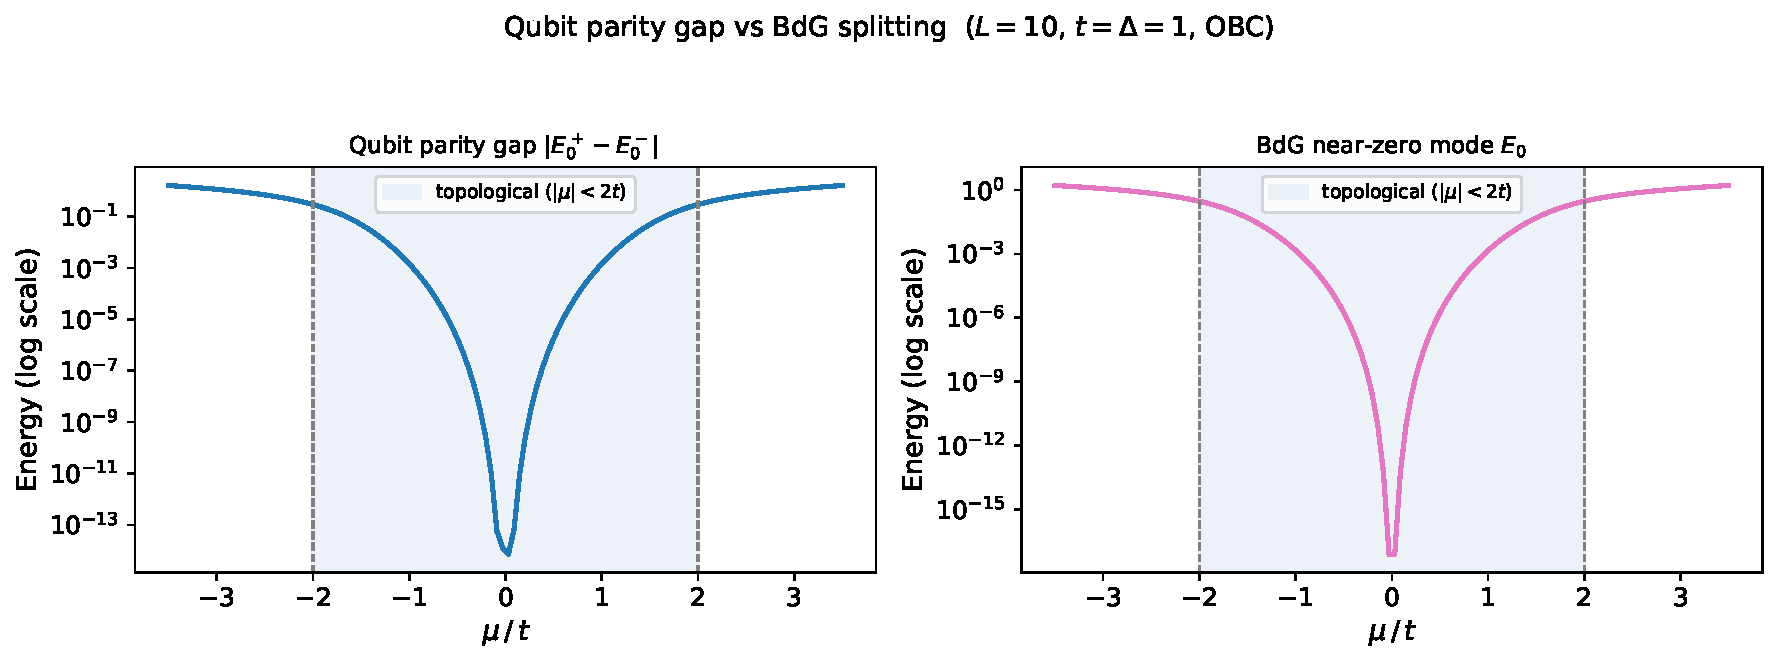
\includegraphics[width=\linewidth,height=0.65\textheight,keepaspectratio]{block2_01_parity_gap_vs_bdg.pdf}
  \end{center}
  Both methods give the same exponential decay in the topological phase and
  the same gap size in the trivial phase — confirming the JW mapping is exact.
\end{frame}

\begin{frame}{Many-body qubit spectrum}
  \begin{center}
    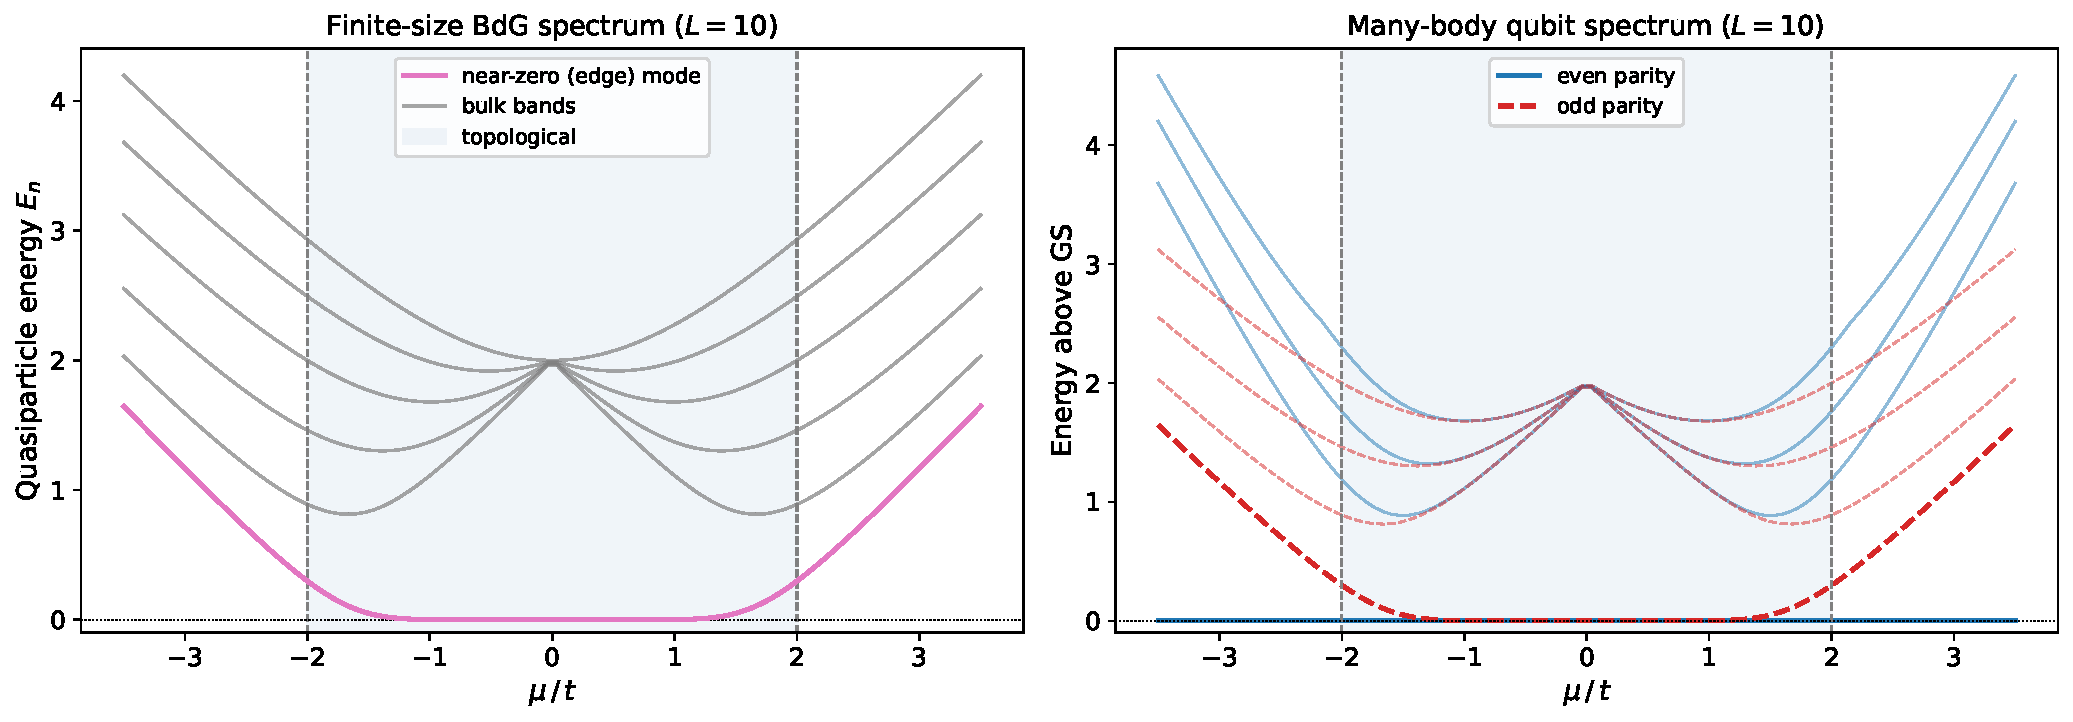
\includegraphics[width=0.82\linewidth,height=0.65\textheight,keepaspectratio]{block2_02_qubit_spectrum.pdf}
  \end{center}
  Even (blue) and odd (red) parity sectors are degenerate inside the
  topological phase and split outside — the bulk-boundary correspondence
  is manifest directly in the many-body spectrum.
\end{frame}

% ══════════════════════════════════════════════════════════════════════════════
\section{Summary}

\begin{frame}{Block 2 — key takeaways}
  \begin{enumerate}
    \item The \textbf{Jordan-Wigner transform} maps fermions to qubits by
          attaching a $Z$-string that restores anticommutation.
    \item The Kitaev Hamiltonian becomes an \textbf{XY model with transverse
          field}: $-\tfrac{\mu}{2}\sum Z_j
          + \tfrac{t-\Delta}{2}\sum XX + \tfrac{t+\Delta}{2}\sum YY$.
    \item \textbf{Fermion parity} $P = \prod Z_j$ is conserved — it
          partitions the spectrum into even/odd sectors.
    \item The \textbf{parity gap} $|E_0^+ - E_0^-|$ is exponentially small
          in the topological phase and of order the bulk gap in the
          trivial phase — a direct qubit-space signature of topology.
    \item Qubit and BdG spectra \textbf{agree exactly} — validating the
          mapping numerically.
  \end{enumerate}
  \vfill
  \textbf{Next (Block 3):} Measuring topology — circuit-based measurements, edge \& string observables.
\end{frame}

\end{document}
